\documentclass[12pt, titlepage]{article}

\usepackage{xcolor} % for different colour comments
\usepackage{tabto}
\usepackage{mdframed}
\mdfsetup{nobreak=true}
\usepackage{xkeyval}
\usepackage{tabularx}
\usepackage{booktabs}
\usepackage{hyperref}
\hypersetup{
    colorlinks,
    citecolor=black,
    filecolor=black,
    linkcolor=red,
    urlcolor=blue
}
\usepackage[singlelinecheck=off, skip=2pt, labelfont=bf]{caption}
\usepackage{titlesec}
\usepackage{graphicx}
\graphicspath{ {image/} }



%% the following adds another section level by redefining the paragraph
%% source:  http://tex.stackexchange.com/questions/60209/how-to-add-an-extra-level-of-sections-with-headings-below-subsubsection
\setcounter{secnumdepth}{4}

\titleformat{\paragraph}
{\normalfont\normalsize\bfseries}{\theparagraph}{1em}{}
\titlespacing*{\paragraph}
{0pt}{3.25ex plus 1ex minus .2ex}{1.5ex plus .2ex}



%% used for counting in event list
\newcounter{EventList}
\newcommand{\printEvent}{
    \stepcounter{EventList}
    \arabic{EventList}.
}

%% used for counting in phase list
\newcounter{PhaseList}
\newcommand{\printPhase}{
    \stepcounter{PhaseList}
    \arabic{PhaseList}.
}



%% Comments
\newif\ifcomments\commentstrue

\ifcomments
\newcommand{\authornote}[3]{\textcolor{#1}{[#3 ---#2]}}
\newcommand{\todo}[1]{\textcolor{red}{[TODO: #1]}}
\else
\newcommand{\authornote}[3]{}
\newcommand{\todo}[1]{}
\fi

\newcommand{\wss}[1]{\authornote{magenta}{SS}{#1}}
\newcommand{\ds}[1]{\authornote{blue}{DS}{#1}}



%% The following are used for pretty printing of events and requirements
\makeatletter

\define@cmdkey      [SRS] {req}     {use}       {}
\define@cmdkey      [SRS] {req}     {desc}      {}
\define@cmdkey      [SRS] {req}     {rationale} {}
\define@cmdkey      [SRS] {req}     {orig}      {}
\define@cmdkey      [SRS] {req}     {fit}       {}
\define@cmdkey      [SRS] {req}     {sat}       {}
\define@cmdkey      [SRS] {req}     {dissat}    {}
\define@cmdkey      [SRS] {req}     {priority}  {}
\define@cmdkey      [SRS] {req}     {conf}      {}
\define@cmdkey      [SRS] {req}     {supp}      {}
\define@cmdkey      [SRS] {req}     {hist}      {}

\define@cmdkey      [SRS] {event} {name}      {}
\define@cmdkey      [SRS] {event} {trigger}   {}
\define@cmdkey      [SRS] {event} {precond}   {}
\define@cmdkey      [SRS] {event} {postcond}  {}

\newcounter{EventNum}
\newcommand{\event}[1]{
\setkeys[SRS]{event}{#1}
\refstepcounter{EventNum}
\begin{mdframed}
\noindent {\bf Use Case \#:} \arabic{EventNum}\\[\baselineskip]
\begin{tabularx}{\textwidth}{@{}p{3cm}X@{}}
{\bf Name:} & \cmdSRS@event@name\\
{\bf Trigger:} & \cmdSRS@event@trigger\\
{\bf Precondition:} & \cmdSRS@event@precond\\
{\bf Postcondition:} & \cmdSRS@event@postcond
\end{tabularx}
\end{mdframed}
}


\newcounter{ReqNum}
\newcommand{\req}[1]{
\setkeys[SRS]{req}{#1}
\stepcounter{ReqNum}
\begin{mdframed}
\noindent {\bf Requirement \#:} \arabic{ReqNum} \tabto{4.3cm} {\bf Requirement Type:} \arabic{section}.\arabic{subsection} \tabto{9.8cm} {\bf Use Case:} \cmdSRS@req@use\\[\baselineskip]
\begin{tabularx}{\textwidth}{@{}p{3cm}X@{}}
{\bf Description:} & \cmdSRS@req@desc\\
{\bf Rationale:} & \cmdSRS@req@rationale\\
{\bf Fit Criterion:} & \cmdSRS@req@fit\\[\baselineskip]
\end{tabularx}
\begin{tabularx}{0.5\textwidth}{@{}p{4cm}X@{}}
{\bf Cust. Satisfaction:} & \cmdSRS@req@sat \\
{\bf Priority:} & \cmdSRS@req@priority \\[\baselineskip]
\end{tabularx}
\begin{tabularx}{0.5\textwidth}{@{}p{4.5cm}X@{}}
{\bf Cust. Dissatisfaction:} & \cmdSRS@req@dissat\\
{\bf Conflicts:} & \cmdSRS@req@conf\\[\baselineskip]
\end{tabularx}
\begin{tabularx}{\textwidth}{@{}p{5cm}X@{}}
{\bf Supporting Materials:} & \cmdSRS@req@supp\\
{\bf History:} & \cmdSRS@req@hist
\end{tabularx}
\end{mdframed}}

\makeatother


\begin{document}

\title{\bf Platform Perils\\[\baselineskip]\Large Software Requirements Specification\\[2\baselineskip] \large Based on the Volere Template}
\author{Steven Palmer\\$\langle$palmes4$\rangle$\\Chao Ye\\$\langle$yec6$\rangle$}
\date{\today}
	
\maketitle

\pagenumbering{roman}
\tableofcontents
\listoftables
\listoffigures

\begin{table}[bp]
\caption*{\bf Revision History}
\begin{tabularx}{\textwidth}{p{3cm}p{2cm}X}
\toprule {\bf Date} & {\bf Version} & {\bf Notes}\\
\midrule
October 7, 2015 & 1.0 & Created document\\
October 7, 2015 & 1.1 & Major edits in progress\\
October 8, 2015 & 1.2 & Major event and reqs additions\\
October 9, 2015 & 1.3 & Final version for rev 0 hand-in\\
April 24, 2016 & 1.4 & Final version for rev 1 hand-in\\
\bottomrule
\end{tabularx}
\end{table}

\newpage

\pagenumbering{arabic}
\section{Project Drivers}
\subsection{The Purpose of the Project}
The purpose of this project is to produce a game that will be used as a demonstration for students in a third year software engineering game design course at McMaster University.  The game will incorporate the \href{https://chipmunk-physics.net/}{Chipmunk2D} physics library and highlight its capabilities.
\subsection{The Stakeholders}
\subsubsection{The Client}
The client for this project is \href{http://www.cas.mcmaster.ca/~smiths/}{Dr.~Spencer Smith} of the Computing and Software department at McMaster University.
\subsubsection{The Customers}
The customers for this project are students who will take the game design course in the future.
\subsubsection{Other Stakeholders}
Other stakeholders include future instructors of the game design course or other similar courses, and future developers of the game.

\newpage
\section{Project Description}
\subsection{Game Overview}
For this project a 2.5-D game will be created.  It will consist of a game world within which a user-controlled hero makes progress by completing stages.  The subsections that follow provide a more detailed explanation of the game.

\subsubsection{The Story}
Platform Perils focuses on a nameless hero who finds himself lost in a world full of dangerous hazards.  It is up to the player to help the hero navigate safely through a series of perilous stages so that he can return home.

\subsubsection{Game Theme}
The game will be a fast-paced platformer game, in which the player must reach the end of stages without being killed.  The game will have an adventure theme reminiscent of Indiana Jones, and will include spears, spikes, and boulders that must be avoided by the player.

\subsubsection{Game Style}
The game will utilize 2.5-D graphics and will have a semi-realistic style.  This will be achieved through the use of textures and simulated lighting effects.

\subsubsection{The Hero}
The hero is the protagonist of the game, and is controlled by the user.  The hero is able to move left or right, and to jump, in order to progress through the game.  The hero can interact with different objects in the game.  These objects include platforms, obstacles, and hazards.  When the hero comes into contact with an object a collision event is triggered.  Depending on the type of object, these events include:

\begin{enumerate}
  \item If the object is a platform, the hero is supported (if standing on) or blocked (if jumping from below)
  \item If the object is an obstacle the hero will be stopped and unable to pass.
  \item If the object is a fatal hazard, the hero will be killed.
\end{enumerate}



\subsection{Mandated Constraints}

The project is subject to several constraints.  The following constraints are mandated by the client:

\begin{enumerate}
  \item The game must make significant use of the Chipmunk2D physics library.
  \item Project milestones must be completed by the dates given in the CS 4ZP6 syllabus.
  \item The project must be fully completed by April 25, 2016.
\end{enumerate}

The following constraints are mandated by the developers:

\begin{enumerate}
  \item User inputs devices are limited to a mouse and keyboard.
\end{enumerate}


\subsection{Naming Conventions and Terminology}
The terminology used in this project is given in \hyperref[tab:terminology]{Table~\ref*{tab:terminology}}.
\begin{table}[h]
\caption{List of terminology} \label{tab:terminology}
\begin{tabularx}{\textwidth}{p{3cm}X}
\toprule {\bf Term} & {\bf Definition}\\
\midrule
Bounds & The boundaries inside which game play occurs\\
Hazard & An environmental object that causes negative effects to the hero\\
Hero & The main character of the game controlled by the user\\
Obstacle & A barrier that the hero cannot cross\\
Surface & An object the hero can stand on (e.g. platforms)\\
User & Player of the game\\
\bottomrule
\end{tabularx}
\end{table}

\begin{table}[ht]
\caption{List of constants} \label{tab:constants}
\begin{tabularx}{\textwidth}{p{3cm}p{2cm}X}
\toprule {\bf Constant} & {\bf Value} & {\bf Description}\\
\midrule
$\sigma$ & 60 & Frame rate target\\
$\Theta$ & 6 & User testing entertainment target\\
$\Psi$ & 2 & User testing challenge range\\
$\Omega$ & 8 & User testing controls target\\
\bottomrule
\end{tabularx}
\end{table}

\newpage
\section{Functional Requirements}
\subsection{The Scope of the Work and the Product}

\subsubsection{The Context of the Work}
A context diagram of the the work is given in \hyperref[fig:context]{Figure~\ref*{fig:context}}.

\begin{figure}[hb]
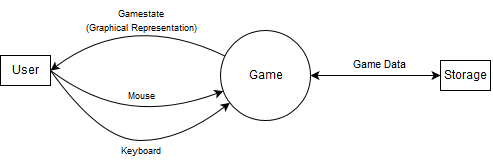
\includegraphics[width=\textwidth]{context}
\caption{Context diagram of the work} \label{fig:context}
\end{figure}


\subsubsection{Work Partitioning}
The flow diagram in \hyperref[fig:gameflow]{Figure~\ref*{fig:gameflow}} gives a rough representation of the operation of the envisioned game.  The user interfaces include a main menu as well as an in-game menu, and an in-game interface in which all game play takes place.  The events are listed in \hyperref[tab:events]{Table~\ref*{tab:events}}.
\begin{figure}
\includegraphics[width=\textwidth]{game_flow}
\caption[Flow diagram of the game]{Flow diagram of the game.  Ovals represent user interfaces and rectangles represent events.} \label{fig:gameflow}
\end{figure}

\begin{table}
\caption{List of events} \label{tab:events}
\begin{tabularx}{\textwidth}{p{0.5cm}>{\raggedright}p{3cm}>{\raggedright}p{3.5cm}>{\raggedright\arraybackslash}X}
\toprule & {\bf Event Name} & {\bf Inputs/Outputs} & {\bf Summary}\\
\midrule
\printEvent & Select Stage & User Input (in) & A stage is started\\
\printEvent & Exit to Main Menu & User Input (in) & Exit from current game to main menu\\
\printEvent & Move Hero & User Input (in) Gamestate (out) & The hero moves through the game world\\
\printEvent & Adjust View & User Input (in) Gamestate (out) & The view of the stage is changed\\
\printEvent & Hero Contacts Surface & Gamestate (out) & The hero comes into contact with a surface\\
\printEvent & Hero Contacts Obstacle & Gamestate (out) & The hero comes into contact with an obstacle\\
\printEvent & Hero Contacts Hazard & Gamestate (out) & The hero comes into contact with a hazard\\
\printEvent & Hero is Killed & Gamestate (out) & The stage resets\\
\printEvent & Stage is Completed & Gamestate (out) & The\\
\printEvent & Exit Game & User Input (in) & The game application is terminated\\
\bottomrule
\end{tabularx}
\end{table}

\subsubsection{Individual Product Use Cases}

Due to the nature of the project, the product use cases are essentially equivalent to the events identified in the work partitioning.

\event{
    name = Select Stage,
    trigger = The user selects to play a stage,
    precond = The stage select menu is open,
    postcond = The selected stage is loaded and play begins from a designated starting point
} \label{event:selectlevel}

\event{
    name = Exit to Main Menu,
    trigger = The user selects to exit to main menu,
    precond = The user is currently playing a stage,
    postcond = The stage is ended and the main menu is opened
} \label{event:exittomain}

\event{
    name = Move Hero,
    trigger = Inputs from user related to controlling the hero movement,
    precond = The user is currently playing a stage,
    postcond = Hero moves according to input
} \label{event:movehero}

\event{
    name = Adjust View,
    trigger = Inputs from user related to controlling the view,
    precond = The user is currently playing a stage,
    postcond = View changes according to input
} \label{event:adjview}

\event{
    name = Hero Contacts Surface,
    trigger = Hero comes into contact with a surface,
    precond = The user is currently playing a stage,
    postcond = Hero is affected by the surface
} \label{event:herosurface}

\event{
    name = Hero Contacts Obstacle,
    trigger = Hero comes into contact with an obstacle,
    precond = The user is currently playing a stage,
    postcond = Hero is affected by the obstacle
} \label{event:heroobstacle}

\event{
    name = Hero Contacts Hazard,
    trigger = Hero comes into contact with hazard,
    precond = The user is currently playing a stage,
    postcond = Hero is affected by the hazard
} \label{event:herohazard}

\event{
    name = Hero is Killed,
    trigger = Hero contacts fatal hazard,
    precond = The user is currently playing a stage,
    postcond = The stage is reset and the hero is moved to the designated starting point
} \label{event:herodefeated}

\event{
    name = Stage is Completed,
    trigger = Hero contacts the goal,
    precond = The user is currently playing a stage,
    postcond = The user is returned to the main menu
} \label{event:levelcompleted}

\event{
    name = Exit Game,
    trigger = The user selects exit game,
    precond = The main menu is open,
    postcond = The application is terminated
} \label{event:exitgame}

\subsection{Functional Requirements}

\req{
        use = \ref{event:selectlevel},
        desc = The user shall have the ability to select a stage to play,
        rationale = The user must be able to play stages of the game,
        fit = Stages are able to be selected for play,
        sat = 1,
        dissat = 5,
        priority = Medium,
        conf = None,
        supp = None,
        hist = {Updated April 24, 2016}
}

\req{
        use = \ref{event:selectlevel},
        desc = The game shall have three predefined levels,
        rationale = The game is designed to have three levels,
        fit = The game supports the selection of three levels,
        sat = 3,
        dissat = 3,
        priority = Medium,
        conf = None,
        supp = None,
        hist = {Created April 24, 2016}
}

\req{
        use = \ref{event:selectlevel},
        desc = The game shall load stages by parsing level scripts at run-time,
        rationale = The game must support loading custom levels,
        fit = The game successfully loads levels from level scripts,
        sat = 5,
        dissat = 1,
        priority = Low,
        conf = None,
        supp = None,
        hist = {Created April 24, 2016}
}

\req{
        use = \ref{event:exittomain},
        desc = The user shall have the ability to exit the current game,
        rationale = The user requires a method of quitting a game in progress,
        fit = User is able to exit the current game and return to the main menu,
        sat = 1,
        dissat = 5,
        priority = Low,
        conf = None,
        supp = None,
        hist = {Created October 9, 2015}
}

\req{
        use = \ref{event:movehero},
        desc = The user shall be able to move the hero to the left,
        rationale = The hero must be able to be moved left to navigate the game world,
        orig = Steven Palmer,
        fit = The hero moves left correctly based on specific user inputs,
        sat = 3,
        dissat = 5,
        priority = Very High,
        conf = None,
        supp = None,
        hist = {Created October 8, 2015}
}

\req{
        use = \ref{event:movehero},
        desc = The user shall be able to move the hero to the right,
        rationale = The hero must be able to be moved right to navigate the game world,
        orig = Steven Palmer,
        fit = The hero moves right correctly based on specific user inputs,
        sat = 3,
        dissat = 5,
        priority = Very High,
        conf = None,
        supp = None,
        hist = {Created October 8, 2015}
}

\req{
        use = \ref{event:movehero},
        desc = The user shall be able to make the hero jump when standing on a surface,
        rationale = The hero must be able to jump to reach the intended areas of the game world,
        fit = The hero is able to jump based on a specific user input,
        sat = 3,
        dissat = 5,
        priority = Very High,
        conf = None,
        supp = None,
        hist = {Created October 8, 2015}
}

\req{
        use = \ref{event:movehero},
        desc = The user shall not be able to make the hero jump when not standing on a surface,
        rationale = The hero must only be able to jump from surfaces,
        fit = The hero is unable to jump when not standing on a surface,
        sat = 3,
        dissat = 3,
        priority = High,
        conf = None,
        supp = None,
        hist = {Created April 24, 2016}
}

\req{
        use = \ref{event:movehero},
        desc = The hero shall be subject to the laws of physics,
        rationale = The game world's laws of physics should apply to the hero,
        fit = The hero's movement responds appropriately to the laws of physics,
        sat = 5,
        dissat = 5,
        priority = High,
        conf = None,
        supp = None,
        hist = {Created October 9, 2015}
}

\req{
        use = \ref{event:movehero},
        desc = The hero shall remain in bounds,
        rationale = The hero must remain in the intended boundaries of play for the game to function properly,
        fit = Hero is unable to pass through walls and other obstacles,
        sat = 2,
        dissat = 5,
        priority = Medium,
        conf = None,
        supp = None,
        hist = {Created October 7, 2015}
}

\req{
        use = \ref{event:movehero},
        desc = All intended areas of the game shall be reachable,
        rationale = All areas of the game where the hero is intended to be should be reachable,
        fit = All areas reachable when testing,
        sat = 2,
        dissat = 5,
        priority = Medium,
        conf = None,
        supp = None,
        hist = {Created October 7, 2015}
}

\req{
        use = \ref{event:adjview},
        desc = The user shall be able to zoom the view of a stage in,
        rationale = The user should be able to zoom in to improve stage navigation,
        orig = Steven Palmer,
        fit = The stage view is zoomed in based on specific user input,
        sat = 2,
        dissat = 3,
        priority = Low,
        conf = None,
        supp = None,
        hist = {Created April 24, 2015}
}

\req{
        use = \ref{event:adjview},
        desc = The user shall be able to zoom the view of a stage out,
        rationale = The user should be able to zoom out to get a better idea of the big picture of the stage,
        orig = Steven Palmer,
        fit = The stage view is zoomed out based on specific user input,
        sat = 2,
        dissat = 3,
        priority = Low,
        conf = None,
        supp = None,
        hist = {Created April 24, 2015}
}

\req{
        use = \ref{event:herosurface},
        desc = The hero shall be supported when standing on surfaces,
        rationale = The hero should be able to stand on surfaces,
        fit = The hero is supported by surfaces,
        sat = 3,
        dissat = 5,
        priority = Medium,
        conf = None,
        supp = None,
        hist = {Created April 24, 2016}
}

\req{
        use = \ref{event:heroobstacle},
        desc = The hero's movement shall be obstructed when he comes into contact with an obstacle,
        rationale = Obstacles should stop the hero,
        fit = The hero cannot pass through obstacles,
        sat = 3,
        dissat = 4,
        priority = Medium,
        conf = None,
        supp = None,
        hist = {Created April 24, 2016}
}

\req{
        use = \ref{event:herohazard},
        desc = The hero shall be killed when he comes into contact with a fatal hazard,
        rationale = Hazards are fatal,
        fit = The hero is defeated,
        sat = 3,
        dissat = 3,
        priority = Medium,
        conf = None,
        supp = None,
        hist = {Created April 24, 2016}
}

\req{
        use = \ref{event:herodefeated},
        desc = The current stage shall be reset when the hero is killed,
        rationale = The user begins from the beginning of the current stage when the hero is defeated,
        fit = The stage resets when the hero is defeated,
        sat = 1,
        dissat = 3,
        priority = High,
        conf = None,
        supp = None,
        hist = {Updated April 23, 2016}
}

\req{
        use = \ref{event:levelcompleted},
        desc = The user shall return to the main menu when a stage is complete,
        rationale = The user must be able to complete stages,
        fit = The user is returned to the main menu upon the hero reaching the goal,
        sat = 1,
        dissat = 3,
        priority = High,
        conf = None,
        supp = None,
        hist = {Updated April 23, 2016}
}

\req{
        use = \ref{event:exitgame},
        desc = The user shall have the ability to exit the application,
        rationale = The user must be able to terminate the game when done playing,
        fit = User is able to successfully terminate application,
        sat = 1,
        dissat = 2,
        priority = Low,
        conf = None,
        supp = None,
        hist = {Created October 8, 2015}
}

\newpage
\section{Non-functional Requirements}
\subsection{Look and Feel Requirements}
\req{
        use = N/A,
        desc = The game shall use 2.5-D graphics,
        rationale = The game is intended to be a 2.5-D game,
        fit = 2.5-D graphics are used for the game,
        sat = 5,
        dissat = 5,
        priority = Low,
        conf = None,
        supp = None,
        hist = {Updated April 24, 2016}
}

\req{
        use = N/A,
        desc = The game shall be a fast-paced platformer with an Indiana Jones adventure theme,
        rationale = The game is intended to be an adventure platformer game,
        fit = The game is an adventure platformer type of game,
        sat = 4,
        dissat = 3,
        priority = Low,
        conf = None,
        supp = None,
        hist = {Created April 24, 2016}
}

\req{
        use = N/A,
        desc = The game theme shall have a semi-realistic aesthetic,
        rationale = The game is intended to have a semi-realistic aesthetic,
        fit = The game incorporates textures and lighting that provide semi-realism to objects,
        sat = 3,
        dissat = 3,
        priority = Low,
        conf = None,
        supp = None,
        hist = {Created April 24, 2016}
}

\req{
        use = N/A,
        desc = The game shall include sounds that enhance the feel of the game,
        rationale = The game is intended to have background music and sound effects,
        fit = The game incorporates background music and sound effects,
        sat = 3,
        dissat = 3,
        priority = Low,
        conf = None,
        supp = None,
        hist = {Created April 24, 2016}
}

\subsection{Usability and Humanity Requirements}
\req{
        use = N/A,
        desc = The game shall be entertaining,
        rationale = A game should be fun,
        fit = The game should be ranked at least $\hyperref[tab:constants]{\Theta}$ for entertainment based on a usability study,
        sat = 5,
        dissat = 5,
        priority = Medium,
        conf = None,
        supp = None,
        hist = {Created October 7, 2015}
}

\req{
        use = N/A,
        desc = The game controls shall be intuitive,
        rationale = The game should be easy and intuitive to control,
        fit = The game should be ranked at least $\hyperref[tab:constants]{\Omega}$ for intuitive controls based on a usability study,
        sat = 3,
        dissat = 5,
        priority = Medium,
        conf = None,
        supp = None,
        hist = {Created October 7, 2015}
}

\req{
        use = N/A,
        desc = The game shall be moderately challenging,
        rationale = A game should be moderately challenging,
        fit = The game should be ranked 5$\pm\hyperref[tab:constants]{\Psi}$ for entertainment based on a usability study,
        sat = 3,
        dissat = 3,
        priority = Medium,
        conf = None,
        supp = None,
        hist = {Created October 7, 2015}
}

\subsection{Performance Requirements}
\req{
        use = N/A,
        desc = The game shall maintain an average framerate of at least $\hyperref[tab:constants]{\sigma}$ fps,
        rationale = A framerate of $\hyperref[tab:constants]{\sigma}$ fps or greater will ensure smooth animation,
        fit = The game runs at $\hyperref[tab:constants]{\sigma}$ fps or greater when testing,
        sat = 5,
        dissat = 5,
        priority = High,
        conf = None,
        supp = None,
        hist = {Created October 7, 2015}
}
\subsection{Operational and Environmental Requirements}
There are no operational and environmental requirements related to this project.
\subsection{Maintainability and Support Requirements}
\req{
        use = N/A,
        desc = {The game shall support Windows, Linux, and OS X operating systems},
        rationale = Students use a variety of operating systems,
        fit = The game compiles and runs on each operating system,
        sat = 5,
        dissat = 3,
        priority = High,
        conf = None,
        supp = None,
        hist = {Created October 7, 2015}
}
\subsection{Security Requirements}
There are no security requirements related to this project.
\subsection{Cultural Requirements}
\req{
        use = N/A,
        desc = {The game shall use the English language},
        rationale = Students at McMaster University are expected to speak English,
        fit = The game uses proper English free of spelling and grammar errors,
        sat = 1,
        dissat = 3,
        priority = Low,
        conf = None,
        supp = None,
        hist = {Created October 7, 2015}
}
\subsection{Legal Requirements}
There are no legal requirements related to this project.

\newpage
\section{Project Issues}
\subsection{Open Issues}
There are no open issues at this time.

\subsection{Off-the-Shelf Solutions}
Pre-existing open-source games developed using Chipmunk2D could be considered off-the-shelf solutions for this project.  These games include \href{http://www.findbestopensource.com/product/ognom-keeper}{Ognom-keeper}, \href{http://www.findbestopensource.com/product/kineticart}{Kineticart}, \href{http://www.findbestopensource.com/product/sole-scion}{Sole-scion}, and several others.  Developing a custom game, however, allows the game to be tailor-made for use as a classroom example.

\subsection{New Problems}
No new problems are expected to arise as a result of this project.
\subsection{Tasks}
The project will be broken down into the phases given in \hyperref[tab:phases]{Table~\ref*{tab:phases}}.
\begin{table}[h]
\caption{List of project phases} \label{tab:phases}
\begin{tabularx}{\textwidth}{p{0.5cm}>{\raggedright}p{4.5cm}X}
\toprule & {\bf Phase Name} & {\bf Summary}\\
\midrule
\printPhase & Interfaces & Programming game interfaces (i.e. working menu systems).\\
\printPhase & Structures & Programming of game structures and classes.\\
\printPhase & Mechanics & Programming of game mechanics including physics implementation.\\
\printPhase & Graphics and Sound & Addition of textures and sound to the game to provide an enhanced audiovisual experience.  This phase is non-crucial. \\
\bottomrule
\end{tabularx}
\end{table}
\subsection{Migration to the New Product}
There is no product being replaced, and thus no migration is required.
\subsection{Risks}
The successful completion of the project depends on overcoming the following significant risks:
\begin{enumerate}
  \item In order to use the Chipmunk2D library it must first be successfully compiled.  Since we intend for the game to be compatible with Windows 7, Mac OS X, and Ubuntu, there is a significant risk for the project to fail if compilation is not achieved on all three operating systems.
  \item Chipmunk2D is a large library and its use is not straight forward.  Successful implementation of the library features is crucial to the success of the project and the failure of this poses another significant risk.
\end{enumerate}
\subsection{Costs}
There are no costs associated with this project.
\subsection{User Documentation and Training}
User documentation will be created as per the CS~4ZP6 guidelines.  No training will be required.
\subsection{Waiting Room}
There are no backlogged requirements at this time.  
\subsection{Ideas for Solutions}
There are no ideas for solutions at this time.  
\end{document}
